\chapter{Implementation Details} \label{implementationDetails}

\section{Introduction to AMBER and NEXMD}

AMBER is primarily known as a classical force-field molecular dynamics package.
It's a massive project maintained by people across the globe that's been designed to work with extensive systems ranging in the tens of thousands of atoms. \cite{case2020a}
AMBER can use a huge range of simulations from replica-exchange to study ph-dependent conformation changes to QM/MM umbrella sampling using nudge elastic bands. \cite{cruzeiro2020exploring, ghoreishi2019fast,sarkar2019ph}
AMBER is a package that contains many smaller programs. One of these programs, SANDER, originally an acronym for Simulated Annealing with Nmr-Derived Energy Restraints, is one of the main engines for running molecule dynamic simulations. 
Most importantly for this research, it has a proven track record of doing QM/MM solvent-solute simulations using periodic boundary conditions.
It has been designed to perform the QM/MM calculations using various libraries specializing in QM calculations as a backend. But by default, it uses the Semi-empirical Quantum Mechanic (SQM) package. These libraries only need to find the forces and energies of the QM region. Note that these packages will still need to know the presence of MM atoms to treat them as external point charges. SANDER will perform the rest of the QM/MM interaction calculations as well as the coordinate propagation. No work has yet been done to allow excited-state dynamics to be performed with SANDER.

NEXMD, currently being developed by the Tretiak lab in Los Alamos, has a proven track record of performance on stimulating ultra-fast non-adiabatic behaviors.
Its ability to solve the state coupling equations on-the-fly has found great utility for systems with hundreds of atoms.
Numerous studies have implemented the research method into topics, including the study of chlorophyll organic conjugated molecules and \(\pi\) conjugated macrocycles.  \cite{zheng2017photoinduced,nelson2014nonadiabatic,alfonso2016interference,wu2006exciton,Ondarse-Alvarez2016}
Such studies with NEXMD have, thus far, been limited to implicit solvents.
No method to provide NEXMD with QM/MM capabilities have yet to be implemented.
The current iteration of NEXMD relies on a modified version of the same SQM library that SANDER uses as its backend. This allows NEXMD to more naturally share state with SANDER and make it a prime candidate for SANDER's gaining excited-state and non-adiabatic dynamics capabilities.

\section{Schematics}
\noindent
\begin{minipage}[c]{\textwidth}
  \centering
  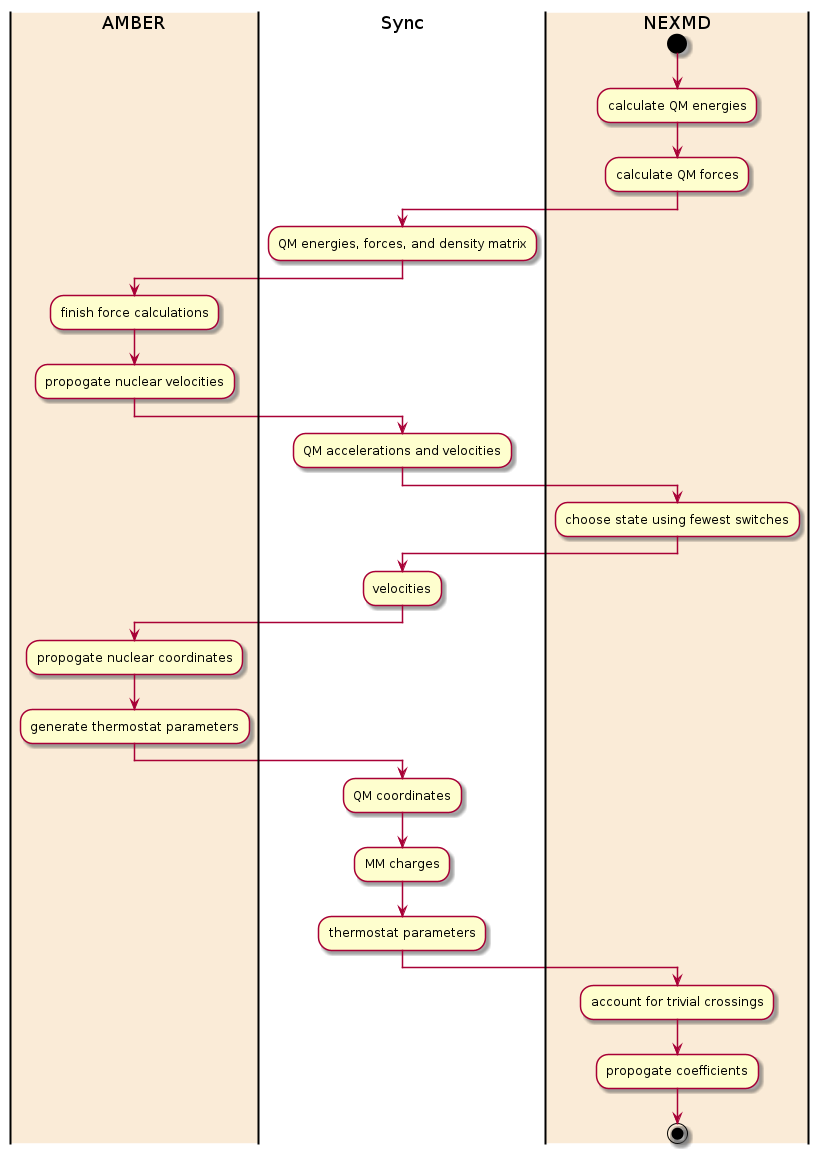
\includegraphics[width=0.7\linewidth]{../Paper2/scripted_diagrams/nasqm_overview.png}
  \captionof{figure}{Swim-lane diagram describing the common time-step of the SANDER-NEXMD interface.}
  \label{scheme:nasqm}
\end{minipage}\bigskip

The swim-lane chart in figure \ref{scheme:nasqm} describes a
common time-step that occurs within the SANDER-NEXMD
interface. With the coordinates provided by SANDER, NEXMD will
calculate and return to SANDER the energies and forces on the QM
atom and the excited-state density. With these results, SANDER
performs the final section of the QM/MM procedure as well as
determines the forces due to classical force fields to derive
the accelerations and velocities for the classical time-step. NEXMD then decides whether to perform a state transition
using the fewest switches algorithm, adjusting velocities as
needed to conserve energy. SANDER then propagates the nuclear
coordinates and generates a new set of random thermostat
parameters. NEXMD then checks if any trivial crossing occurs
within the potential energy surfaces. Once proper accounting
between the PESs and the energy order is determined, NEXMD
propagates the quantum coefficients.

When users initiate SANDER, they provide the usual SANDER inputs of coordinate,
parameter, and sander control files. An example of a SANDER ctrl file is shown in Figure
\ref{fig:ctrl}.

   \lstset{frame=single}
   \begin{mylisting}
     An example SANDER input file
     &ctrl
       ntx=5,
       ntb=1,
       ig=-1,
       taup=2.0,
       cut=16.0,
       tempi=300.0,
       temp0=300.0,
       ntt=3,
       gamma_ln=20.0,
       nstlim=2000,
       dt = 0.0005,
       ifqnt=1,
     /
     &qmmm
       scfconv=1.0E-8,
       qmmask=`:1',
       nae=1 ! Flag that links to NEXMD
     /
   \end{mylisting}
   \captionof{figure}{Example SANDER ctrl file for the SANDER-NEXMD interface}\label{fig:ctrl}
   \bigskip
   \setlength\parindent{24pt}
This file contains all the information regarding molecular dynamics, excluding most of the QM
calculations and all of the nonadiabtic parameters and is a standard input file to the AMBER
molecular dynamics programs.

To use NEXMD, the user will include the flag NAE under the QM/MM section of the input
file. This flag causes SANDER to call the NEXMD versions of the QM/MM force calculations instead of the default SQM routines. With the NEXMD force routine called, NEXMD will then look for the primary input file used in the stand-alone version of NEXMD, the input.ceon file. An example of this file is included below.

\lstset{frame=single}
\begin{mylisting}
&qmmm
    !***** Ground-State and Output Parameters
    qm_theory=`AM1', ! Integral type 
    verbosity=1, ! QM/MM output verbosity
    !***** Excited-State Parameters
    exst_method=1, ! CIS (1) or RPA (2) [1]
    dav_guess=1, ! Restart Davidson from (0) Scratch, (1) Previous,
    printcharges=1, ! (1) Print Mulliken Charges [0]
    !***** Solvent Models and External Electric Fields
    solvent_model=0, ! (0) None,
&endqmmm
&moldyn
    !***** General Parameters
    natoms=12, ! Number of atoms
    rnd_seed=19345, ! Seed for the random number generator bo_dynamics_flag=0, ! (0) Non-BO or (1) BO [1]
    exc_state_init=2, ! Initial excited-state (0 - ground state) [0]
    n_exc_states_propagate=3, ! Number of excited-states [0]
    !***** Dynamics Parameters
    n_quant_steps=4, ! Number of quantum steps for each classical step [4]
    num_deriv_step=1.0d-3, ! Displacement for numerical derivatives, A [1.0d-3]
    rk_tolerance=1.0d-7, ! Tolerance for the Runge-Kutta propagator [1.0d-7]
    !***** Non-Adiabatic Parameters
    decoher_type=2, ! (2) At successful plus frustrated hops...
    quant_step_reduction_factor=2.5d-2, ! Quantum step reduction factor [2.5d-2]
    !***** Thermostat Parameters
    therm_type=1, ! (1) Langevin | IGNORED,
    therm_temperature=300, ! Thermostat temperature, K | IGNORED
    therm_friction=20, ! Thermostat friction coefficient, 1/ps | IGNORED
    !***** Output & Log Parameters
    verbosity=3, ! NEXMD output verbosity (0-minimum, 3-maximum)
    out_data_steps=1, ! Number of steps to write data [1]
    out_coords_steps=10, ! Number of steps to write the restart file [10]
    out_data_cube=0, ! Write (1) or do not write (0) view files to generate cubes [0]
    out_count_init = 0, ! Initial count for view files [0]
&endmoldyn
&coord
    ! IGNORED
&endcoord
&veloc
    ! IGNORED
endveloc
&coeff
    0.00 0.00
    1.00 0.00
    0.00 0.00
&endcoeff
\end{mylisting}
%% \captionof{figure}{Example NEXMD input.ceon file for the SANDER-NEXMD interface}%\label{fig:inputceon}
\bigskip

Users can find additional flags and their corresponding options in the
NEXMD and AMBER documentation. The input.ceon file contains the
majority of the flags and preferences for the QM calculation and all
the non-adiabatic choices. The namespace QMMM exists in both the SANDER
ctrl file and the NEXMD input.ceon file. Both NEXMD and SANDER read
this namespace is into a shared struct due to NEXMD using SQM as a
backend; however, their respective parsers will look for different
flags. The SANDER parser will run first and will need the three flags
shown in \ref{fig:ctrl} to call the NEXMD routines. The NEXMD parser
for the QMMM namespace will then override anything else included in
both input files’ QM/MM namespace.

No modification to the input.ceon file is necessary from the stand-alone NEXMD code to run with SANDER. However, the coordinates
and velocities included in the file will be ignored, since SANDER
manages these data points. SANDER reads the coordinates and velocities
through the standard SANDER parameter and coordinates files
instead. Users can decide to leave these sections blank or to include
them, whatever their convenience. The preferences in the input.ceon file include the number
of QM steps between any classical time-step, the number of excited
states to include in the CIS calculation, the initial state, and the
initial coefficients. Note that a portion of this input file, such as
the thermostat preferences, relates to coordinate dynamics. SANDER
controls dynamics and will override these settings during
runtime. Users may want to remove these preferences from the
input.ceon file to avoid any confusion.

With the coordinates at time t = 0, NEXMD can calculate the energies in
a similar method described in Chapter 2. NEXMD is capable of
performing these energy calculations using Time-Dependent
Hartree-Fock, Time-Dependent Density Functional theory, or CIS. In
this work, we focus on the use of CIS. NEXMD can perform CIS
calculations using any of the semi-empirical methods available in SQM.
AM1 provides very reasonable computational cost to accuracy for our
systems of interest. It is the de-factor semi-empirical Hamiltonian
for organic conjugated molecules such as the one we will analyze in
chapters 4 and 5 \cite{silva2010benchmark} An analysis of parameter
choices can be found in previous
literature.\cite{nelson2012nonadiabatic} During the ground state
energy and density calculations, NEXMD heavily relies on slightly
modified SQM routines. These calculations follow the same principles
as described in the QM/MM section of Chapter 2. However,
unlike that section, we do not adequately account for the QM charges
during the QM-Ewald calculation. Proper treatment would require
multiple iterations of both the ground state SCF and the excited-state
Davidson algorithm. Further details of this problem as well as a
recommended solution can be found in the future works section of
Chapter 6. \cite{Walker2008} For a general time-step QM/MM interaction
will be added to the density matrix as follows:
\begin{enumerate}
\item Calculate the MM Ewald potentials using the classical charges
  from the MM atoms.
\item Construct the Hamiltonian matrix as if the QM region was in
  vacuum.
\item Add the one-electron terms for the interaction between QM
  atoms and the MM atoms within the cutoff to the Hamiltonian.
\item Within the SCF routine, copy the Hamiltonian to the Fock
  matrix and add the QM/MM two-electron integrals. When using AM1,
  SANDER expands the QM charge density into the STO-6G minimal
  basis set while treating the MM atoms as point charges, thereby
  providing the full electrostatic interaction between the QM and
  MM atoms.
\item Calculate the QM Ewald potential using the iteration’s
  Mulliken charges, then add the Ewald potentials for both QM and
  MM atoms to the Fock Matrix. Note that these Mulliken charges will be incorrectly from the ground state.
\item The SCF procedure continues until convergence resulting in a
  density matrix that incorporates solvents.
\end{enumerate}

NEXMD uses this ground-state density to perform a Davidson
diagonalization routine to determine the excited-state
energies. NEXMD then calculates the QM-QM forces using Equation
\ref{eq:NEXMDForces}. With the forces calculated, SANDER then
propagates the velocities by a single time-step. SANDER does not
yet adjust coordinates since NEXMD could still change these
velocities in the upcoming steps.

With the accelerations and velocities passed in by SANDER, NEXMD
then chooses to hop using the Tully fewest switches surface
hopping technique described in Chapter 2. If a hop occurs, NEXMD
adjusts the velocities in the non-adiabatic coupling vector’s
direction to conserve energy. If no hop occurs, then these
velocities remain unchanged.  Decoherence is then managed based
on user preferences. The current fully supported decoherence
methods are to either break coherence at any successful hop or to break at
any time where there is a high non-adiabatic coupling. Users may
also choose to ignore any decoherence correction.

We want to emphasize that at no point does SANDER know of the
multiple adiabatic states. SANDER simply propagates based on the forces and
velocities sent to it. SANDER then uses these new velocities to update
the atomic coordinates, which completes its time-step. SANDER then
begins a new time-step, generates a new set of thermostat parameters,
and forwards the new coordinates and parameters to NEXMD. NEXMD then
checks whether any trivial crossing occurred between the potential
energy surfaces by comparing the electron density matrices’ overlap.
\cite{nelson2012nonadiabatic} With the PESs correctly accounted for,
NEXMD then propagates the coefficients numerically using the
Runge-Kutta-Verner fifth-order and sixth-order method with the
coefficients described as
\begin{align}
  c_\alpha &= \sigma_\alpha e^{i\theta \alpha}\\
  \dot{\sigma}_\alpha &= - \sum_{\beta} \sigma_{\beta} \cos(\theta_{\beta} - \theta_{\alpha}) \dot{\mathbf{R}} \cdot \mathbf{d_{\alpha\beta}}\\
  -\hbar \sigma_\alpha \dot{\theta}_\alpha &= \sigma_\alpha \text{E}_\alpha + \hbar \sum_\beta \sigma_\beta \sin(\theta_{\beta} - \theta_\alpha)\dot{\mathbf{R}} \cdot \mathbf{d_{\alpha\beta}}.
\end{align}
NEXMD uses code developed by Hull, Enight, and Jackson to perform this calculation.\cite{hull1996runge}
Solvents are accounted for in the calculation of the Fock matrix during the ground-state SCF calculations. The non-adiabatic coupling terms are calculated numerically using Equation \ref{eq:NACouplingTerm}. The time derivative of the Fock matrix is determined using the differences of the elements between time-steps. This propagation does not require the calculation of intermediary forces.
Accurately calculating the non-adiabatic coupling terms requires a smaller time-step than what is necessary for nuclear coordinate propagation, and as such, we separate time-steps into smaller quantum time-steps. We use a procedure developed by Tully and Hammes-Schiffer to determine the chance of performing a hop over multiple time-steps.\cite{hammes1994proton}
In their work, they showed that
\begin{equation}
  g_{\alpha\beta} = \frac{\sum_j^{N_q} b_{\beta\alpha}(j) \delta t}{a_\alpha\alpha},
\end{equation}
where the number of intermidiary quantum steps per classical
propogation of the nuclear coordinates is described by \(N_q\). We
would need to calculate n(n-1) non-adiabatic coupling terms had we
allowed for more than a single hop to occur between time-steps. With
reasonable time-steps, the likelihood of more than a single hop
happening is extremely low; thus, we forbid the occurrence. This
restriction allows us to calculate only the non-adiabatic coupling from
the current excited-state.

In our work, we use four quantum time-steps for every classical time
step. Previous works demonstrate this as a reasonable number to use
for these parameters.\cite{nelson2012nonadiabatic} During each of
these quantum time-steps, NEXMD must calculate the energies and
non-adiabatic coupling terms. These calculations require interpolation
of the nuclear coordinates between the two classical time-steps. To
perform this interpolation, SANDER must pass the coordinates,
velocities, accelerations, and thermostat parameters to
NEXMD. However, this transfer is not very straightforward since NEXMD
uses a different time-step procedure than SANDER. For clarity, we will
first only look at the case of Newtonian mechanics without
excited-state transitions. When SANDER begins, it calculates a single
point calculation at time t = 0 and uses the calculated forces to
propagate the velocities (v) 1/2 a time-step (\(\delta\)) back. In its
main loop, it reperforms the energy and force calculation at time
t = 0. SANDER uses those accelerations to propagate v(t=-\(\delta\)/2) a
single time-step, making it the average velocity between t = 0 and
t=\(\delta\). It then moves the coordinates a time-step using this
average velocity. We show these coupled equations in equations
\ref{eq:SANDERNewtonian} and \ref{eq:SANDERNewtonian2}.

\begin{align}
  v(\delta/2) &= v(-\delta/2) + a(0)\delta \label{eq:SANDERNewtonian}\\
  x(\delta) &= x(0) + v(\delta/2) \delta \label{eq:SANDERNewtonian2}
\end{align}

NEXMD performs a theoretically equivalent algorithm but with numerical
differences. NEXMD calculates the energies and forces at t = 0 to move
the coordinates an entire time-step and the velocities a
half-time-step. It then calculates the acceleration for t = \(\delta\) using the
coordinates at t = \(\delta\) with which it uses to propagate the velocities the
last half of the time-step.
\begin{align}\label{eq:NEXMDNewtonian}
  x(\delta) &= x(0) + v(0)\delta + 1/2 a(0) \delta^2 \\
  v(\delta/2) &= v(0) + a(0)\delta/2\\
  v(\delta) &= v(\delta/2) + a(\delta)\delta/2
\end{align}
NEXMD does not calculate the energies and forces at time t = 0 twice as
performed in SANDER. The SCF calculation uses the previously
calculated density matrix for its initial guess. Because SANDER will
perform, at minimum, two iterations during an SCF calculation, the
forces and energies produced by NEXMD for the first step will differ
slightly from those produced by SANDER even though they use the same
SCF routines. These small differences between the two programs in the
first step will lead to larger differences later. However, both
programs still return qualitatively identical results.

SANDER never calculates the velocities between time-steps.  As such,
the half-step velocities needed by NEXMD for the calculations of the
non-adiabatic coupling vectors and the interpolation of the QM steps
need to be the average of the old and new velocities in SANDER.

Using the Langevin thermostat, NEXMD will also require the generated
random variables for the thermostat generated by AMBER to determine
the stochastic forces used in the QM
interpolation.\cite{paterlini1998constant} In AMBER, the Langevin
thermostat is accounted for in the coordinate propogation
\begin{align}
  x(\delta) &= x(0) + v(\delta/2) t\\
  x(\delta) &= x(0) + \left(v(-\delta/2) c_e + (F(0) + R(0)) \frac{c_i \delta}{m} \right) \delta,
\end{align}
where \(F(0)\) is the force at t = 0, m the mass of the atom, and
\(R(0)\) a random perturbation generated by a gaussian distribution
dependent on the temperature, atom mass, time-step and friction
coefficient.  The coefficients \(c_e\) and \(c_i\) are based of the
Langevin friction coefficient \(\gamma\)
\begin{align}
  c_e &= 1 - \frac{\gamma\delta}{2}\\
  c_e &= \frac{1}{1 + \frac{\gamma \delta}{2}}.
\end{align}
In NEXMD, the Langevin equations are also included in the coordinate propogation but as
\begin{align}
  x(\delta) = x(0) + (v'(0)\chi_v + a'(0)\chi_a + P_r),
\end{align}
where \(\chi_v\), \(\chi_a\), and \(P_r\) are the fricition, intertia,
and stochastic forces repectively.  The prime indicates the variable
is in atomic units as opposed to the units used in SANDER.

This can be expanded to 
\begin{align}
  x(\delta) = x(0) + ((v'(-\frac{\delta}{2}) + \frac{1}{2}a'(0)\chi_v + V_r(-\delta))\chi_v + a'(0)\chi_a + P_r),
\end{align}
where \(V_r\) is a random perturbation to the velocities.
\(\chi_v\) and \(\chi_a\) are non-random variables and can be generated by NEXMD by feeding NEXMD the Langevin friction coefficient \(\gamma\).
With a bit of algebra, the convertion from SANDER to NEXMD for the random variable can be derived to be
\begin{align}
  V_r &= \frac{1}{2}(v(\delta/2) - v(-\delta/2))\nu_{an} - \frac{1}{2}a'(0)\chi_v\\
  P_r &= v(\delta/2)) - \left( \frac{1}{2} (v(-\delta/2) + v(\delta/2))\nu_{an}\chi_v + a'(0)\chi_a \right),
\end{align}
where \(\nu_{an} \approx 9.35E-4\) is a unit convertion from SANDER to NEXMD.

Once the quantum coefficients are propogated, the cycle continues with
the calculations of the QM/MM energies.

\section{Benchmarks}
    \noindent
    \begin{multiFigure} 
      \addFigure{0.45}{./Images/Timings/bo_npropogated}
      \addFigure{0.45}{./Images/Timings/bo_nsolvents}
      \captionof{figure}[Adiabatic timings]{Run time per time-step for PPV\(_3\)-NO\(_2\) with 3254 explicit methanol solvents during adiabatic dynamics.}
      \label{fig:adiabaticTimings}
    \end{multiFigure}\bigskip

    \noindent
    \begin{multiFigure} 
      \addFigure{0.45}{./Images/Timings/nbo_npropogated}
      \addFigure{0.45}{./Images/Timings/nbo_nsolvents}
      \captionof{figure}[Non-adiabatic timings]{Run time per time-step for PPV\(_3\)-NO\(_2\) with 3254 explicit methanol solvents during non-adiabatic dynamics.}
      \label{fig:nonadiabaticTimings}
    \end{multiFigure}\bigskip



Figures \ref{fig:adiabaticTimings} and \ref{fig:nonadiabaticTimings} show the timings for the Sander-NEXMD interfaces. 
Benchmarks consisted of a single PPV\(_3\)-NO\(_2\) molecule surrounded by 3254 CH\(_3\)OH molecules.
PPV\(_3\)-NO\(_2\) consists of 50 atoms, and every additional CH\(_3\)OH molecule adds 6 atoms for 19,754 atoms total.
We vary both the number of solvents included in the QM region and the number of excited-states propagated.
We performed these calculations on an AMD Ryzen 5 3600XT. Results are averaged over 8 trajectories. The initial coordinates and velocities for these 8 trajectories were sampled from a 320 ps ground state MM trajectory. Each datapoint shares these same initial conditions. Each trajectory ran for 30 0.5 fs time-steps, and the results are averaged over time.

Non-adiabatic trajectories requires roughly an order of magnitude more computational time than the corresponding adiabatic cases. Increasing the number of states increases the computational costs nearly linearly, as expected for configuration interaction calculations. The computational costs for adding solvents into the QM region increase superlinearly, expected while using semi-empirical methods. Therefore, we are limited in the number of solvents we can include in the QM region and will need to be selective in which we choose.

Results for ground-state QM/MM dynamics using the SANDER-NEXMD interface were identical to those with SANDER using the default SQM library with and without using a thermostat. This is due to NEXMD using this same SQM library for a backend. Results from the interface for non-adiabatic dynamics in vacuum are nearly identical to those produced from NEXMD alone. A minor difference occurs due to SANDER performing the initial energy and force calculations twice while NEXMD only performs it once. For single-point calculations, these results are identical.
